% !TeX root = ../slides.tex
\subsection{Figures}

\begin{frame}[t]{Figure Recommendations}


\vspace{1em}
\begin{minipage}{0.49\textwidth}
\centering
{\small\textbf{(a)} \only<1>{Example figure}\only<2>{Policy Starts in 2015}} \\
\only<1>{\includegraphics[width=\textwidth]{example-image-golden}}%
\only<2>{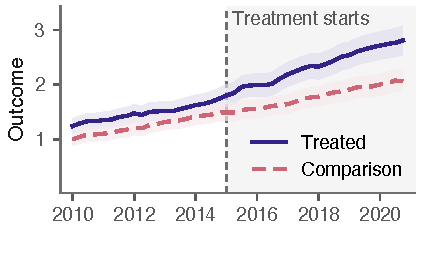
\includegraphics[width=\textwidth]{figures/example_group_means}}%
\end{minipage}
\hfill
\only<2->{%
\begin{minipage}{0.49\textwidth}
\centering
{\small\textbf{(b)} Difference-in-Differences Estimator} \\
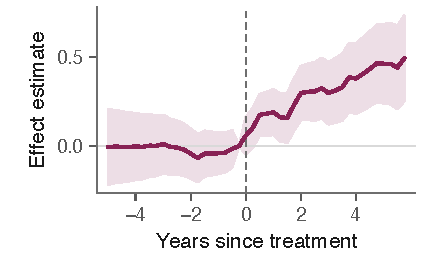
\includegraphics[width=\textwidth]{figures/example_did}%
\end{minipage}%
}%
\vspace{1em}

\begin{itemize}
\item Export figures in golden-ratio proportions (e.g., $6.5\times4$ inches). 
\item<2->[\textcolor{accent}{$\rightarrow$}] Two of them fit side by side and leave space for the explanation and the \myuline{punchline}!
\end{itemize}

\end{frame}

